\section{SMC model} \label{sec:smc_model}
After having produced the best trace from the \gls{cora} model, we get a trace that contains descriptions of when different payloads are executed. These instruction is given to the \gls{smc} model along with relevant information from the global config like battery settings, schedule length etc.

Since \gls{smc} allows for non-linear priced automata along with rational number this allow us to use \gls{kibam} which was discovered during \cref{sec:kibam}, The advantage of using this model over the others in that section is that \gls{kibam} is pessimistic in the sense that \gls{kibam} tends to underestimate the actual battery levels. This leads to \gls{kibam} being the preferred model to used in the \gls{smc} model.

Our \gls{smc} model consist of four templates plus some additional template instance depending on the number of windows described in the input format. For the moment there need to be at least one window defined in the input. This makes a total of at least 5 templates, which are Processor, Insolation, EnergySource, Scheduler, and OrbitWindows. 
The overall model is in large part taken from \cite{battery_aware_scheduling}. It covers scheduling with uncertainty combined with capturing battery levels during execution of the schedule. The rest of this section we will go over each of the important changes and addition we made to the model, this include the concept of recharging, windows for payload, and dependencies for payloads. 

The bases of these template are based of \cite{battery_aware_scheduling}, which construct a \gls{smc} model, to run payloads with a \gls{kibam} battery model where each payload had a best, worst, deadline, earliest release time, and latest release time to describe the payloads running times and deadline. We initially already had a concept of best and worst running time but added the deadline parameter based on this paper. Because it would ensure that no payload would interfere with each other no matter how fast the payload finished. This is done in the processor template that describes what payload is current in the process of being execute. The first payload is set during the transition to the \uppLoc{Wait} location from the \uppLoc{Init} location, here it waits the appropriate amount of time depending on the RunStart variable which is an array of all the starting time for each payload gathered from the \gls{cora} model. After the waiting period has passed it then enter the \uppLoc{Ready} location to indicate the payload it ready to be executed, and from there it continues to the \uppLoc{Running} location when the scheduler template broadcast the run channel. From there it stays between the best and worst running time of the particular payload which is gathered from the payload description. The last location \uppLoc{Idle} indicate that the payload has finished and it is now waiting to pass the time until its ultimate deadline also described in the payload description. If it is the last payload in the schedule it takes the transition leading to the location \uppLoc{Done}.

\begin{figure}[H]
	\centering
	\begin{tikzpicture}
	%Locations
	\node [init] (l0) {$\cup$};
	\node [location] (l1) [right of=l0, xshift=40mm, label={
		[align=left]above:
		\textcolor{name}{Wait}},
	label={
		[align=center]below:
		\textcolor{invariant}{totalTime <= RunStart[payloadNumber]}
	}] {};
	\node [location] (l2) [right of=l1, xshift=80mm, label={
		[align=left]above:
		\textcolor{name}{Ready}
	}] {};
	\node [location] (l3) [below of=l0, yshift=-40mm, label={
		[align=left]below:
		\textcolor{name}{Done}
	}] {};
	\node [location] (l4) [below of=l1, yshift=-40mm, label={
		[align=left]below:
		\textcolor{name}{Idle}\\
		\textcolor{invariant}{x <= D}
	}] {};
	\node [location] (l5) [below of=l2, yshift=-40mm, label={
		[align=left]below:
		\textcolor{name}{Running}\\
		\textcolor{invariant}{x <= W}
	}] {};
	\path[->,black, thick] (l0) edge node [midway, above][align=left]{
		\textcolor{update}{t=0,i = IIdle,}\\
		\textcolor{update}{setActive()}} (l1);
	\path[->,black, thick] (l1) edge node [midway, above][align=center]{
		\textcolor{guard}{totalTime >=RunStart[payloadNumber]}\\
		\textcolor{sync}{ready!}\\
		\textcolor{update}{x=0, t=0,}\\
		\textcolor{update}{deadline()}} (l2);
	\path[->,black, thick] (l2) edge node [midway, right][align=left]{
		\textcolor{sync}{run?}\\
		\textcolor{update}{x := 0,}\\
		\textcolor{update}{setActive(),}\\
		\textcolor{update}{enqueue()}\\
		\textcolor{update}{earnings += Profit[active]}} (l5);
	\path[->,black, thick] (l4) edge node [midway, left][align=left]{
		\textcolor{sync}{skip?}\\
		\textcolor{update}{payloadNumber ++,}\\
		\textcolor{update}{skipped()}} (l2);
	\path[->,black, thick] (l5) edge node [midway, below][align=left]{
		\textcolor{guard}{x >= B}\\
		\textcolor{update}{dequeue(), active = -1,}\\
		\textcolor{update}{payloadNumber ++}} (l4);
	\path[->,black, thick] (l4) edge node [midway, left][align=left]{
		\textcolor{guard}{x >= D \&\&}\\
		\textcolor{guard}{!done()}\\
		\textcolor{update}{setActive()}} (l1);
	\path[->,black, thick] (l4) edge node [midway, below][align=left]{
		\textcolor{guard}{done()}\\
		\textcolor{update}{on = false,}\\
		\textcolor{update}{active = -1}} (l3);
	\end{tikzpicture}
	\caption{Processor template}
	\label{fig:smc_P}
\end{figure}

When the location \uppLoc{Ready} from Processor is active, two transitions is available to either execute or skip the current payload, each of the transition is depending on the scheduler template seen in \cref{fig:smc_S}. This template from the paper is in charge of determine if a payload can be run based on the battery levels, they would calculate what the expected a would be after the payload have been executed. This is also something we needed have to ensure that a payload does not draw more power then was currently available, but additional guards is needed to check for dependencies, windows and battery threshold, all of these checks are done on the transition that broadcast \uppSync{run!} indicating that it is safe to execute the payload. If for some reason we are not able to perform the transition it waits until we either have recharged enough energy or window are correct for the payload, if we are not able to perform the payload within time, which is calculated by subtracting worst from the payload deadline, then the other transition in this model is performed leading to a skip of the payload. With dependencies this can have major consequences because the next payload in the schedule may have depended the payload thus creating a chain of skipped payloads.

\begin{figure}[H]
	\centering
	\begin{tikzpicture}
	%Locations
	\node [init] (l0) {};
	\node [location] (l1) [right of=l0, xshift=40mm, label={
		[align=left]right:
		\textcolor{invariant}{t <= Payloads[Queue[payloadNumber]][2] - }\\
		\textcolor{invariant}{Payloads[Queue[payloadNumber]][1]}
	}] {};
	\path[->,black, thick] (l1) edge[bend left=50] node [midway, below][align=left]{
		\textcolor{guard}{t == Payloads[Queue[payloadNumber]][2] - }\\
		\textcolor{guard}{Payloads[Queue[payloadNumber]][1]}\\
		\textcolor{sync}{skip!}
	} (l0);
	\path[->,black,thick] (l0) edge node [midway, below][align=left]{
		\textcolor{sync}{ready?}} (l1);
	\path[->,black,thick] (l1) edge[bend right=45] node [midway, above][align=left]{
		\textcolor{guard}{on \&\& mayRun() \&\&}\\
		\textcolor{guard}{0.1 < a * exp(-k2*W)+}\\
		\textcolor{guard}{(((a+b)*k2*c-(IPayload+IIdle))*(1.0-exp(-k2*W))}\\
		\textcolor{guard}{-(IPayload+IIdle)*c*(k2*W-1.0+exp(-k2*W)))/k2}\\
		\textcolor{guard}{\&\& Threshold < checkB(a,b,totalTime)}\\
		\textcolor{sync}{run!}\\
		\textcolor{update}{runs[active] ++,}\\
		\textcolor{update}{totalRuns[active] ++}
	} (l0);
	\end{tikzpicture}
	\caption{Scheduler template}
	\label{fig:smc_S}
\end{figure}

The OrbitWindows template can be found in \cref{fig:smc_OW}, with three location and circular transition. When the first transition from the initial location is taken, means that the windows is now active by changing the variable \uppVar{inWindow[id]} to one the \uppVar{id} is used to access the array depending on the active template \jfx{oliver er dette den korrekte måde at beskrive id formål?}. When time has passed and window is no longer inside the window the next transition is taken, lastly when a full orbit has been performed it resets the clock \uppVar{wtime}.

During the entire schedule we need to keep track of battery level, this is done with \gls{kibam} as mentioned in that start of this section which was also used by the paper. It would need to calculate the values of \uppVar{a} and \uppVar{b}, and enable the battery model to recharge. Only the calculation of \uppVar{a} and \uppVar{b} was usable from the paper. So to add the capability of recharging a new location is added to ensure that \uppVar{b} can not exceed it value based on the total capacity, so when the model entered the new location it would not add the values of recharge to b. Additionally a guard is set on the transition leading back to \uppLoc{Charging}, that says \uppVar{b} needs to be drained a small amount of power before going back to the initial location. This is done to prevent damaging the battery further. The final template can be found in \cref{fig:smc_ES}

With these changes to the \gls{smc} model we are able to run a schedule with payloads, that have windows and dependencies, with the capability of recharging the battery based on the Insolation tempalte found in \cref{fig:smc_I}, now we only need to consider what queries that should be performed in order to give the most usable data for the users.


%Where the \gls{cora} model finds a trace, the \gls{smc} model will try and rerun the produced trace. This means the \gls{smc} model will execute tasks in the exact same order as the \gls{cora} model.% As this model implements KiBaM it gives a fairly accurate representation of the energy consumption. 

%\Cref{fig:cost_schedule} and \cref{fig:solar_task}, shows the different templates used in the \gls{smc} model. To the left of \cref{fig:cost_schedule} are the energy source. The energy source is responsible for updating the remaining available and bound energy, and in case there are no more available energy, it will synchronise with the scheduler which will then stop running more tasks.
%On the right of \cref{fig:cost_schedule} is the scheduler, it awaits a synchronisation from the tasks in order to ensure that they are ready for execution. The scheduler then estimates if running another task will deplete the battery. If this is the case it will transition back to the initial location preparing to run another task. If running another task would not deplete the battery, the task will be run.

%\begin{figure}[H]%
%	\centering
%	\subfloat
%	{{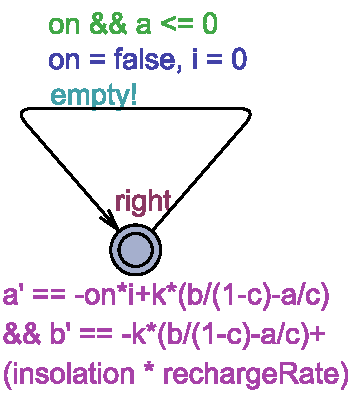
\includegraphics[width=4cm]{graphics/smc_costhandler.pdf} }}%
%	\qquad
%	\subfloat
%	{{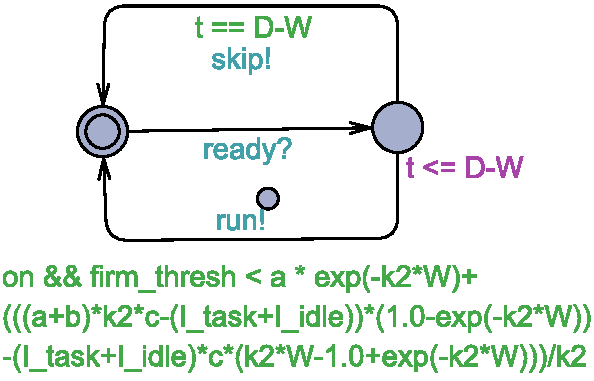
\includegraphics[width=6cm]{graphics/smc_scheduler.pdf} }}%
%	\caption{The \gls{smc} model's energy source(left) and scheduler(right)}%
%	\label{fig:cost_schedule}%
%\end{figure}

%On the left side of \cref{fig:solar_task}, we see the template for the orbit time. It is here assumed that the satellite will spend half its orbit in insolation where it is possible to recharge the battery. It switches the variable \uppVar{Insolation} between true and false, which is used in the calculation of the bound energy.\afx{Kom tilbage hertil når at kibam afsnittet er frdigt. Uddyb om hvordan vores mplementation reflektere teorien fra \cref{sec:kibam}}\\
%The right side of \cref{fig:solar_task} is the template for a task, this indicates that a task can be, ready to be run, running, and inactive. When a task is not running the consumption is lower as indicated by \uppVar{i = I\_idle} which represents the background load of other minor tasks that are not modelled.

%\begin{figure}[H]%
%	\centering
%	\subfloat
%	{{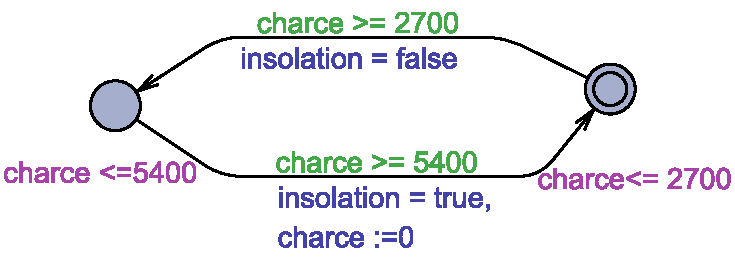
\includegraphics[width=8cm]{graphics/smc_solar.pdf} }}%
%	\qquad
%	\subfloat
%	{{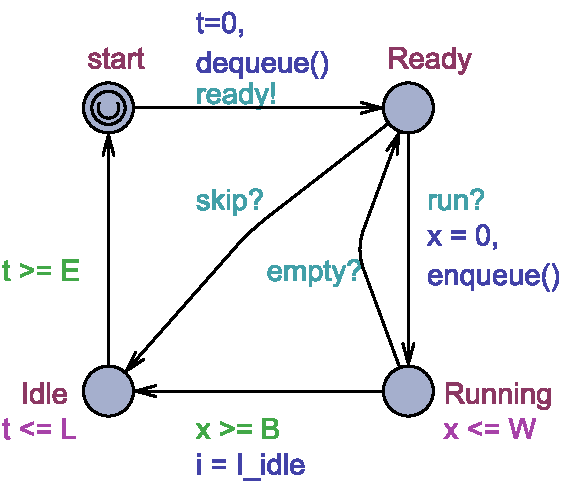
\includegraphics[width=6cm]{graphics/smc_task.pdf} }}%
%	\caption{The \gls{smc} model's representation of solar panels(left) and a task(right)}%
%	\label{fig:solar_task}%
%\end{figure}
%Since the model is made in UPPAAL \gls{smc} we are able to run statistical queries asking for the chance of the available energy falling below some threshold, or to simply track the value of the bound and available energy over time for some specified amount of runs. Examples of such queries can be seen in \cref{eq:pr_low_a_sim_ab}, which indicates, first the chance that the battery level will fall below $55\, \%$ within $43200$ time units. Assuming the time unit is in seconds the example query is for 12 hours. The other query is a simulation of the avilable and bound energy over the same amount of time.\\
%\begin{align}
%Pr[<= 43200] \quad(a <= (c/100)*55)		\nonumber \\
%simulate \quad 1 \quad [<=432000] \quad \{a,b\} 
%\label{eq:pr_low_a_sim_ab}
%\end{align}

%The advantages of running these queries is, that even though the runs in \gls{cora} conclude that a schedule is viable, the probability query may be able to find that running the trace could lead to energy depletion. Also tacking the state of the battery may help to see the effect of the solar panels and the tasks stress on the battery. This is relevant as one or two repetitions of the schedule may not deplete the battery but perhaps ten would, in such case it may be relevant to change some parameters and run it again.